\section{Test}
\label{sec:Test}

Die zu erstellende Software ist mit Abschluss der Umsetzungsphase fertiggestellt und einsatzbereit. Vor Projektabschluss und -übergabe soll die Software auf ihre Qualität geprüft werden. Es soll darüber hinaus verifiziert werden, dass die Anforderungen des Lastenheftes umgesetzt wurden. Sowohl Qualität, als auch die Umsetzung der Anforderungen werden im Folgenden in einem zweistufigen Praxistest der Software sichergestellt.

Im ersten Schritt wird die Software einem Alphatest unterzogen. Ein Alphatest liegt immer dann vor, wenn die Tests von Personen durchgeführt werden, die an der Entwicklung eines Produktes beteiligt waren, in diesem Fall das Projektteam. In diesem Test werden vor allem die Produktfunktionen des Lastenheftes (siehe Abschnitt \nameref{sec:Lastenheft} auf Seite \pageref{sec:Lastenheft}) überprüft. In diesem Test sollen erste grobe Fehler in Bedienung, Anzeige und Verhalten gefunden werden und es soll zusätzlich sichergestellt werden, dass alle Anforderungen des Auftraggebers umgesetzt sind. Die Tests der Produktfunktionen werden zusätzlich in den vier führenden Browsern\footnote{Quelle: \url{http://www.chip.de}} durchgeführt, um browserübergreifende Funktionalität sicherzuestellen.
Dabei wurden jeweils die Testbereiche Bedienung, Anzeige und Verhalten unterschieden. Das Ergbeniss des durchgeführten Alphatests ist in nachfolgender \abbildung{Alphatest} festgehalten:

\begin{figure}[htb]
\centering
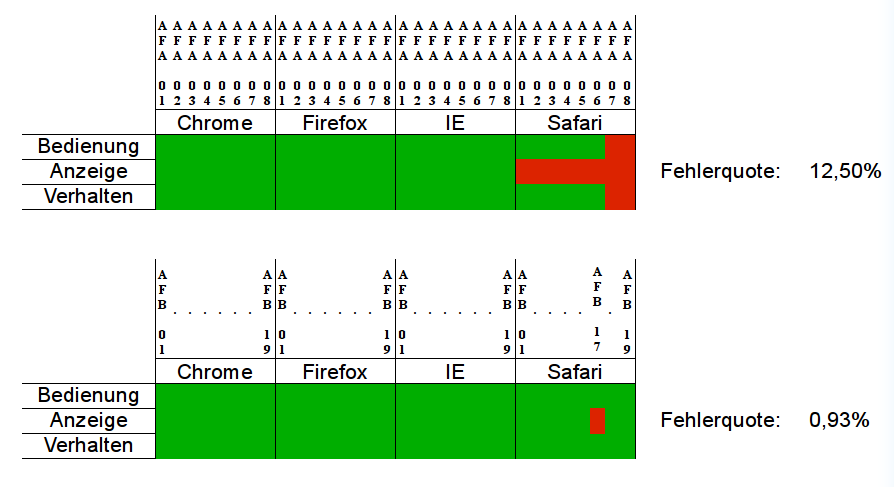
\includegraphics[width=1.0\textwidth]{Alphatest.png}
\caption[Mockup Backend]{Graphische Darstellung des Alphatests\protect\footnotemark}
\label{fig:Alphatest}
\end{figure}
\footnotetext{Quelle: Eigene Darstellung}

Die Auswertung des Alphatests zeigt, dass alle Anforderungen umgesetzt wurden und funktionsfähig sind. Die seperate Betrachtung der vier Internetbrowser zeigt darüber hinaus, dass nicht alle Browser für die Darstellung der Software geeignet sind. Besonders der "`Safari"'-Browser ist für die Darstellung der Anwendersicht nicht geeignet. Bei diesem Browser besteht eine Inkompatibilität zwischen der Technologie der benutzen Google Street View API und der Browserinternen Umsetzung dieser Technologie. Diese Problem lässt sich nicht durch technische Anpassungen innerhalb der Software beheben. Aus diesem Grund wurde beim Aufrufen der Software eine entsprechende Warnung für den Benutzer platziert. Es wird an dieser Stelle darüber hinaus der Google Chrome-Browser für die Verwendung dieser Software empfholen, da dieser, aus subjektiver Betrachtung, die beste Leistung beim Laden und Anzeigen der Inhalte zeigte. Neben browserspezifischen Darstellungsunterschieden konnten in diesem Alphatest auch kleinere Schwachstellen und Fehler gefunden werden, die nicht in den Anwendungsfällen enthalten waren.So zum Beispiel die falsche Verlinkung einer Datei oder das Fehlen einer Sicherheitsabfrage beim Löschen eines Datensatzes. Diese Mängel wurden im Anschluss an den Alphatest direkt beseitigt.